\documentclass[12pt]{article}
\usepackage[utf8]{inputenc}
\usepackage[letterpaper, margin=1in]{geometry}
\usepackage{graphicx}
\usepackage{mathptmx}
\usepackage{float}
\usepackage[cmex10]{amsmath}
\usepackage{amsthm,amssymb}
\usepackage{url}
\urlstyle{same} 
\def\UrlBreaks{\do\/\do-}
\usepackage{breakurl}
\usepackage{fancybox}
\usepackage{breqn}
\usepackage{array}
\usepackage{caption}
\usepackage{subcaption}
\usepackage{comment}
\usepackage[english]{babel}
\usepackage[acronym,nomain]{glossaries} % list of acronyms
\usepackage{xurl}
\usepackage{cite} % math and engineering style citations
\usepackage{multicol}
\usepackage{multirow}
\usepackage{mathptmx}
\usepackage{float}
\usepackage{lipsum}
\usepackage{framed}
\usepackage[T1]{fontenc}
\usepackage[pdfpagelabels,pdfusetitle,colorlinks=false,pdfborder={0 0 0}]{hyperref}

\renewcommand{\arraystretch}{1.2}

\sloppy

\newcolumntype{C}[1]{>{\centering\let\newline\\\arraybackslash\hspace{0pt}}m{#1-2\tabcolsep}}

\title{Time-Varying Optimal Control for Dynamic Systems using Mixed Integer Linear Programming: The Cascading Hydroelectric Reservoir Problem}
\author{Aaron Rabinowitz}
\date{}

\newacronym{chrp}{CHRP}{Cascading Hydroelectric Reservoir Problem}
\newacronym{schrp}{S-CHRP}{Stochastic Cascading Hydroelectric Reservoir Problem}
\makeglossaries

\begin{document}

\maketitle

\section*{Introduction}

This document outlines how to formulate and solve a time-varying optimal controls problem as a linear problem. A linear problem is defined by a linear objective function (in which all terms are linear) and may be bounded and constrained in a non-algebraic manner. A wide variety of solvers are available to solve linear problems with these solvers varying in numerical method. most solvers implement either the Simplex method or Interior Point Optimization. There are also many ways to call the various solvers in various programming languages. Posing an optimization as a Linear problem is useful as it allows for use of the mentioned robust computational infrastructure (Some of the solver methods used for Linear problems can also be used to solve Quadratic problems). In this document and accompanying code repository, examples are given which show how a rather complex optimization problem can be relatively easily solved when posed as a Linear problem.

\subsection*{Direct Transcription into the Time Domain}

Linear and Quadratic problem solvers can only solve a very specific type of problem. The defining features of such a problem are linearly independent decision variables and constraints as linear functions of those design variables. Solving time-varying controls problems with Linear and Quadratic problem solvers requires one to pose the problem in a manner that it can be solved as a Linear or Quadratic problem.

Posing a time-varying optimal controls problem as a Linear or Quadratic problem requires transcription into the time domain. Rather than treating the controls as $N$ time-varying controls ($u=f(t)$), the controls are treated as $N$ sets of $M$ independent variables corresponding to $M$ time-steps ($u=\{u_0,u_1,\dots,u_M\}$). This process, called Direct Transcription, is necessary to pose the problem as a linear problem. The objective function for  continuous and discreet optimization problems are shown in Equations \eqref{eq:exc} and \eqref{eq:exd} respectively.

\begin{equation}
	\min_{u\in U}\quad \int_{t_0}^{t_m}u(t)dt: u=f(t) \label{eq:exc}
\end{equation}

\begin{equation}
	\min_{u\in U}\quad \sum_{k=0}^{M} u_k: u=\{f_0,f_1,\dots,f_M\} \label{eq:exd}
\end{equation}

Once transcribed, the controls at each time-step are independent on one-another which, often, does not represent reality. As an example, one might seek to control the acceleration of a vehicle in order to minimize energy consumption over a given time period. The rate at which the vehicle can change accelerations may be limited physically or by passenger comfort considerations. In this case the relationships between values of the control at different time-steps will have to be enforced by constraints. A possible constraint could be that acceleration at time step $k$ has to be within a certain range centered on acceleration at time-step $k-1$. Adding this constraint will necessitate defining an initial condition which will have influence over the ultimate solution. Such a constraint may take the form

\begin{equation}
	a_{k}-a_{k-1}\leq C \quad k=1,2,\dots,M
\end{equation}

where $C$ is a constant. For the case $k=0$ another constraint will have to be made where $a_{k-1}$ is the inputted constant for initial acceleration. One may also desire to keep track of a problem state which is not a decision variable. For example, in the case of the vehicle mentioned previously, the vehicle may be subject to maximum and minimum speeds. Speed is related to acceleration by the kinematic equation 


\begin{equation}
	v(t)=v(0)+\int_{t_0}^{t_m}a(t)dt \quad \forall m\in \{0,1,\dots,M\}
\end{equation}

where $v$ is velocity and $a$ is acceleration. After transcription, the kinematic equation becomes

\begin{equation}
	v_m=v_0+\sum_{k=0}^{m}a_k\delta t_k \quad \forall m\in \{0,1,\dots,M\}\label{eq:vel_d}
\end{equation}

where $\delta t_k$ is the duration of the  $k^{th}$ time-step. Since Equation \eqref{eq:vel_d} is valid for every possible value of $m$, the value of velocity for each time-step can be found using Equation \eqref{eq:vel_mat}.

\begin{equation}
	\begin{bmatrix}
		v_0 \\ v_1 \\ \vdots \\ v_M
	\end{bmatrix}=
	\begin{bmatrix}
		\delta t_0 & \delta t_1 & \dots & \delta t_M
	\end{bmatrix}
	\begin{bmatrix}
		1 & 0 & \dots & 0\\
		1 & 1 & \dots & 0\\
		\vdots & \vdots &\ddots & \\
		1 & 1 & & 1
	\end{bmatrix}
	\begin{bmatrix}
		a_0 \\ a_1 \\ \vdots \\ a_M
	\end{bmatrix}
	\label{eq:vel_mat}
\end{equation}

Assuming that $a$ is a continuous variable there will be an uncountable infinity of possible combinations of values for the $a$ vector. In all scenarios there will be a corresponding vector of values for the $v$ vector. As can be seen in Equation \eqref{eq:vel_mat}, the relationship between acceleration and velocity is linear and thus, velocity can be a basis for constraints without ever being explicitly defined in the problem.

Another type of non-linearity which may be inherent to an optimization problem is on-off dynamics. As an example, an internal combustion engine requires a certain amount of compression in order to begin the combustion process after which it can operate. There is a band of engine speeds in which the engine can operate below which the power produced by the engine will be too little to compress the air sufficiently for combustion and the engine will stall. Thus there is a discontinuity between 0 and the minimum functional velocity $v^{min}$. The engine will also have a maximum operational velocity of $v^{max}$ In order to model this in a linear manner an \textit{integer} variable will have to be introduced. Integer variables are variables that the solver must keep as integer valued (solvers do this using various methods including branching-and-cutting all of which can seriously increase solver-time). In this case the integer variable will be $e^{on}$ for engine on.
The allowable values for $e^{on}$ will be 0 and 1. The on-off constraints can be written as

\begin{gather}
	e_k^{on}v^{min}-v_k\leq 0 \quad \forall k\in \{0,1,\dots,M\}\label{eq:onoff1}\\
	e_k^{on}v^{max}-v_k\geq 0 \quad \forall k\in \{0,1,\dots,M\}\label{eq:onoff2}
\end{gather}

which forces $v_k=0$ when $e_k^{on}=0$ and $v^{min}\leq v_k\leq v^{max}$ when $e_k^{on}=1$. The previously presented constraint adds one integer variable and thus will increase solver time and should only be included if the discontinuity at 0 is important to results. The on-off constraint may also be insufficient in certain cases where a significant cost is paid in order to change the on-off state. An internal combustion engine requires electric power to run the starter motor to start the engine. When programming a feature such as idle-stop it might be critical to factor this dynamic in. Adding startup and/or shutdown costs for the engine requires two integer variables $e^{startup}$ and $e^{shutdown}$. In this case the on-off state of the engine in the on-off constraint will be a non-explicit state (see Equation \eqref{eq:vel_mat}) and the startup and shutdown costs can be added to the objective function. Opting for startup-shutdown over on-off will increase solver-time.

Finally, one may want to account for nonlinear costs and/or rewards. Continuing with the engine example, internal combustion engines have nonlinear torque curves. The torque curve can be linearized by creating $L$ bounded linear functions representing different regions of the torque curve. As $L$ approaches $\inf$ the linearized functions approach the original nonlinear function. What is needed is a constraint to select the correct linear function based on engine speed to the exclusion of all others. This can be accomplished with a series of on-off constraints (as in Equations \eqref{eq:onoff1} and \eqref{eq:onoff2})for each interval which must collectively sum to 1. With the correct interval selected and all others set to zero the engine torque can be computed as

\begin{equation}
	\eta_k=\sum_{i\in I}[s_im_iv_k+s_ib_i]
\end{equation}

where $\eta$ is engine torque, $i$ is the interval, $m$ is the slope of the linear function on interval $i$, and $b$ is the intercept of the linear function on interval $i$. It is worth noting, as before, that adding interval constraints adds integer variables, one per interval, which will increase solver-time.

\section*{The \gls{chrp}}

\begin{figure}[H]
	\centering
	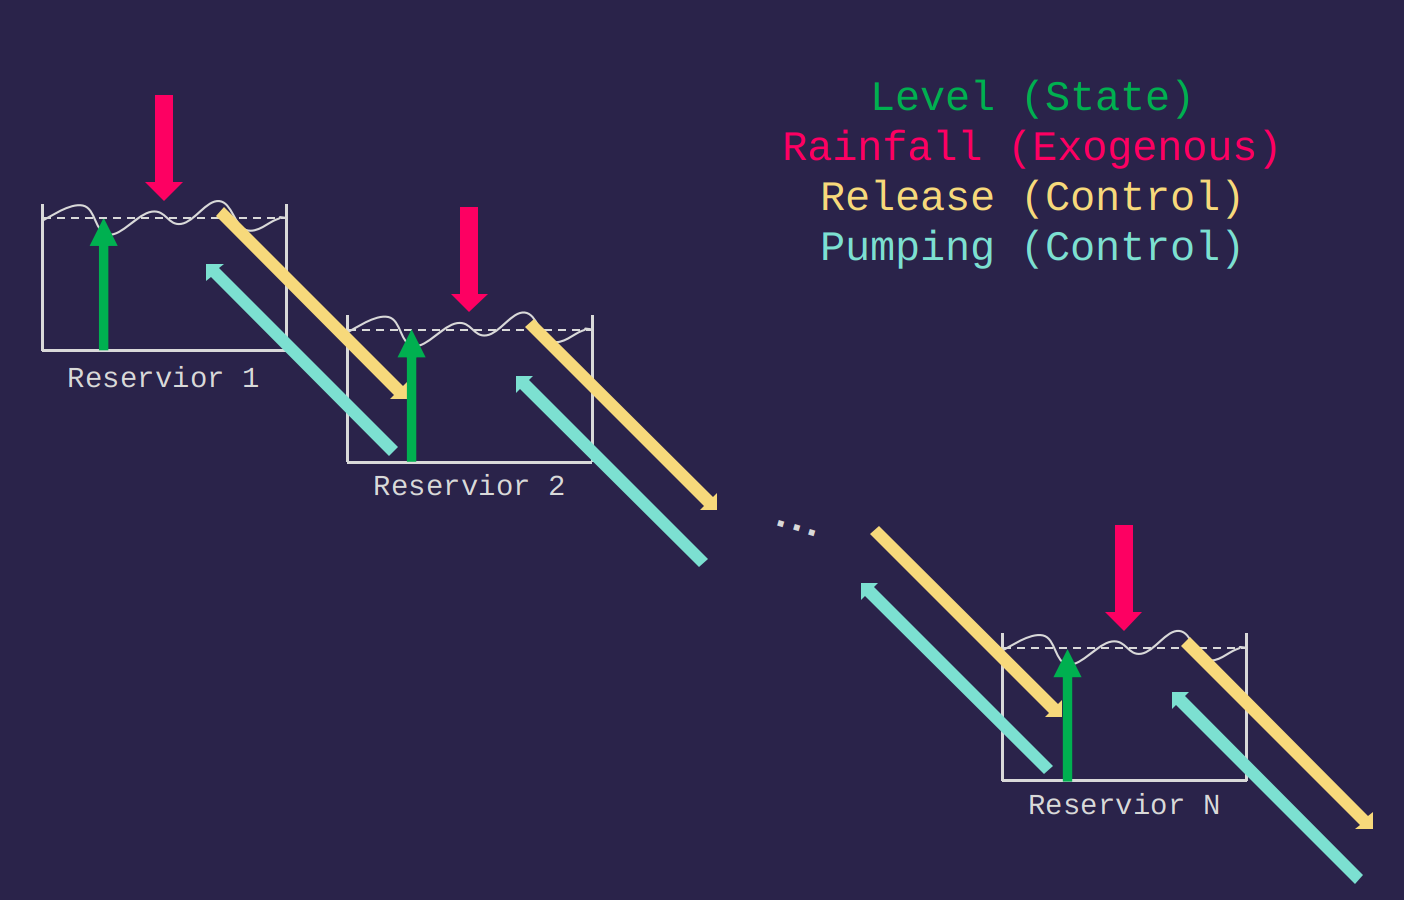
\includegraphics[width=\linewidth]{figs/Schematic.png}
	\caption{Schematic Description of the Problem}
	\label{fig:schematic}
\end{figure}

The \gls{chrp} is a classic example used in the teaching of optimal control and optimization. Formulations of the problem can vary in complexity based on the selection of constraints. In this document a maximalist formulation of the problem is presented with commentary. The purpose of this example is to show how to formulate various types of constraints and how to implement these in code. Deterministic and stochastic formulations are shown separately.

The \gls{chrp} concerns the optimal time-varying control of a series of $N$ interconnected reservoirs gated by hydroelectric dams over $M$ time-steps. The reservoirs are not necessarily of equal capacity. The dams are capable of generating electricity when water is released and capable of pumping water at the cost of expending electricity. Each of the generators and pumps is limited to function within given ranges of flow rates. Generation and pumping power are assumed to be proportional to flow-rate. All reservoirs are subject to rainfall and evaporation (represented as a net flow). Each reservoir level must be maintained within a given range. After reservoir $N$ there is an assumed reservoir of infinite capacity. All reservoirs must be returned to their initial levels at the end of the period of optimization. All reservoirs are connected to the same electricity grid. The grid is also used to provide power for surrounding areas which have a time-varying demand for electricity. The reservoir system operator must meet the local demand and is paid a fixed amount for doing so. If generation is insufficient to meet demand in a given time step then the operator will have to purchase power via transmission. If more power than necessary is produced during a given time period then the excess power may be sold via transmission. The objective of the operator is to maximize profits from the production of electricity by finding optimal time-varying controls for all generators and pumps.

\section*{Deterministic Formulation}

The objective of the problem is to maximize profits. However, it is standard practice to minimize an objective and sometimes this is the only option so the objective will actually be to minimize loss. A negative loss is a profit. In this case the local electricity demand must be met a fixed rate so it does not factor into the optimization. Rather, the optimization only concerns the purchase and sale of power via transmission.

\begin{equation}
	\min_{u\in U}\quad
	\sum_{t\in T}u_{t}^{tp}c_{t}^{tp}+
	\sum_{t\in T}u_{t}^{ts}c_{t}^{ts}
\end{equation}

where $U=[u^g,u^p,u^{tp},u^{ts},u^{gc},u^{pc}]$ is the vector of problem controls containing, in order, generator flow rate, pump flow rate, transmission purchase power, transmission sale power, generator unit commitment, and pump unit commitment, $R$ is the set of reservoirs, $T$ is the set of discrete time-steps of the problem, and $C=[c^g,c^p,c^{tp},c^{ts},c^{gc},c^{pc}]$ is a vector of constant cost multipliers for the problem controls.

Variable definition is fundamental to problem formulation. First, note that $U$ contains multiple variables which are not present in the objective function. These variables are still part of the problem and will show up in the constraints. The variables in $U$ not present in the objective function are able to effect the value of the objective indirectly. Second, note that the number of variables in the problem scales with the number of time steps. Since the solver run-time is expected to scale exponentially with the number of variables, one should endeavor to use the lowest frequency time discretization feasible.

The optimization is subject to the following constraints:

The first constraint is conservation of energy, it is formulated as

\begin{equation}
	\sum_{r\in R}u_{r,t}^{g}-
	\sum_{r\in R}u_{r,t}^{p}+
	u_{t}^{tp}-
	u_{t}^{ts}+
	y_{t}^{e}=0\quad \forall t\in T\label{eq:coe}
\end{equation}

where $y^e$ is the local time-varying power demand and is exogenous. Each reservoir has a range of operation in which its level must be maintained. The operating range lower bound constraint is formulated as

\begin{equation}
	\sum_{t\in T_K}^{L}[u_{r,t}^{g}+u_{r,t}^{p}+y_{r,t}^{f}]\geq LB_{r} : T_K=T_0,T_1,...,T_k \quad\forall k \in 0,1,...,M \quad\forall r \in R \label{eq:lb}
\end{equation}

where $LB$ is the lower boundary of the operating range. This constraint computes the state (reservoir) level for each time step by summing the in and outflows from that reservoir in all previous time-steps. The right hand side of the constraint is equivalent to multiplying an $N$ by $N$ matrix with zeros above diagonal and ones on and below diagonal (called a Lower traingular matrix) by the vectors of in and out flows then summing. A version of this constraint is produced for each reservoir. In matrix form Equation \eqref{eq:lb} would take the form seen in Equation \eqref{eq;mat_lb}.

\begin{equation}
	\begin{bmatrix}
		1 & 0 & \dots & 0\\
		1 & 1 & \dots & 0\\
		\vdots & \vdots &\ddots & \\
		1 & 1 & & 1
	\end{bmatrix}
	\begin{bmatrix}
		u_{r,0}^g \\ u_{r,1}^g \\ \vdots \\ u_{r,N}^g
	\end{bmatrix}+
	\begin{bmatrix}
		1 & 0 & \dots & 0\\
		1 & 1 & \dots & 0\\
		\vdots & \vdots &\ddots & \\
		1 & 1 & & 1
	\end{bmatrix}
	\begin{bmatrix}
		u_{r,0}^p \\ u_{r,1}^p \\ \vdots \\ u_{r,N}^p
	\end{bmatrix}+
	\begin{bmatrix}
		y_{r,0}^f \\ y_{r,1}^f \\ \vdots \\ y_{r,N}^f
	\end{bmatrix}\geq LB_r \quad \forall r \in R
	\label{eq;mat_lb}
\end{equation}

The upper bound constraint is formulated similarly as

\begin{equation}
	\sum_{t\in T_K}^{L}[u_{r,t}^{g}+u_{r,t}^{p}+y_{r,t}^{f}]\leq UB_{r} : T_K=T_0,T_1,...,T_k \quad\forall k \in 0,1,...,M \quad\forall r \in R \label{eq:ub}
\end{equation}

where $UB$ is the upper boundary of the operating range. The final state value is enforced by the constraint

\begin{equation}
	\sum_{t\in T}[u_{r,t}^{g}+u_{r,t}^{p}+y_{r,t}^{f}]=FS_{r} \quad\forall r \in R \label{eq:fs}
\end{equation}

where $FS$ is the final state (level) value for each reservoir. The final constraint is unit commitment. The unit commitment constraint enforces the nonlinear operations of the generators and pumps using two linear variables (one continuous and one binary). The unit commitment constraints are posed as

\begin{gather}
	f_{r,t}^{g,min}u_{r,t}^{gc}-u_{r,t}^{g}\leq 0 \quad\forall r \in R \quad\forall t \in T\\
	f_{r,t}^{g,max}u_{r,t}^{gc}-u_{r,t}^{g}\geq 0 \quad\forall r \in R \quad\forall t \in T\\
	f_{r,t}^{p,min}u_{r,t}^{pc}-u_{r,t}^{p}\leq 0 \quad\forall r \in R \quad\forall t \in T\\
	f_{r,t}^{p,max}u_{r,t}^{pc}-u_{r,t}^{p}\geq 0 \quad\forall r \in R \quad\forall t \in T
\end{gather}

where $f^{g,min}$ and $f^{g,max}$ and the minimum and maximum operating flow rates for each generator and $f^{p,min}$ and $f^{p,max}$ and the minimum and maximum operating flow rates for each pump.

\section*{Stochastic Formulation}

In the deterministic formulation of the problem the exogenous variables, rainfall and local electricity demand are know \textit{a priori}. This is not reflective of real-world operation. There will always be some uncertainty surrounding exogenous variables. In the \gls{schrp} it is assumed that the operator must pass a time-varying transmission schedule to the greater grid dispatch controller before the period of operation in question. The dispatch controller uses this information to optimize the greater grid's coordinated operation and thus, deviations from the agreed transmission schedule are discouraged. In this scenario, the agreed schedule is the baseline and deviations from the agreed schedule are subject to a fee. The job of the reservoir system operator is to provide a transmission schedule which will allow for highest expected profit across a range of scenarios which are not necessarily equally likely to occur.

There are two types of control variables in stochastic programming. Herein these will be called "general" and "specific" variables but they are also called first and second stage variables. General variables are those which apply in all scenarios and specific variables are those which apply in only one scenario. In this problem the transmission schedule is general and the generation, pumping, and transmission controls are all specific.

The objective of the \gls{schrp} is

\begin{gather}
	\min_{u\in U}\quad
	\sum_{t\in T}c_{t}^{tp}u_{t}^{tp}+
	\sum_{t\in T}c_{t}^{ts}u_{t}^{ts}+
	\sum_{s \in S}\sum_{t\in T}p_sc_{t}^{tpd}u_{s,t}^{tpd}+
	\sum_{s \in S}\sum_{t\in T}p_sc_{t}^{tsd}u_{s,t}^{tsd}+
\end{gather}

where $S$ is the set of discrete scenarios considered, $p$ is the probability of each scenario, $u^{tpd}$ and $u_{tsd}$ are the deviations from the transmission schedule for purchasing and selling respectively and $c_{tpd}$ and $c_{tsd}$ are the associated costs. The constraints are:

\begin{equation}
	\sum_{r\in R}u_{s,r,t}^{g}-
	\sum_{r\in R}u_{s,r,t}^{p}+
	u_{t}^{tp}-
	u_{t}^{ts}+
	y_{s,t}^{e}=0\quad \forall s\in S \quad \forall t\in T\label{eq:coe_s}
\end{equation}

\begin{equation}
	\sum_{s \in S}\sum_{t\in T_K}^{L}[u_{s,r,t}^{g}+u_{s,r,t}^{p}+y_{s,r,t}^{f}]\geq LB_{s,r} : T_K=T_0,T_1,...,T_k \quad\forall k \in 0,1,...,M \quad\forall r \in R \quad\forall s \in S \label{eq:lb_s}
\end{equation}

\begin{equation}
	\sum_{s \in S}\sum_{t\in T_K}^{L}[u_{s,r,t}^{g}+u_{s,r,t}^{p}+y_{s,r,t}^{f}]\leq UB_{s,r} : T_K=T_0,T_1,...,T_k \quad\forall k \in 0,1,...,M \quad\forall r \in R \quad\forall s \in S \label{eq:ub_s}
\end{equation}

\begin{equation}
	\sum_{s \in S}\sum_{t\in T}[u_{s,r,t}^{g}+u_{s,r,t}^{p}+y_{s,r,t}^{f}]=FS_{s,r} \quad\forall r \in R \quad\forall s \in S \label{eq:fs_s}
\end{equation}

\begin{gather}
	f_{s,r,t}^{g,min}u_{s,r,t}^{gc}-u_{s,r,t}^{g}\leq 0 \quad\forall r \in R \quad\forall t \in T \quad\forall s \in S\\
	f_{s,r,t}^{g,max}u_{s,r,t}^{gc}-u_{s,r,t}^{g}\geq 0 \quad\forall r \in R \quad\forall t \in T \quad\forall s \in S\\
	f_{s,r,t}^{p,min}u_{s,r,t}^{pc}-u_{s,r,t}^{p}\leq 0 \quad\forall r \in R \quad\forall t \in T \quad\forall s \in S\\
	f_{s,r,t}^{p,max}u_{s,r,t}^{pc}-u_{s,r,t}^{p}\geq 0 \quad\forall r \in R \quad\forall t \in T \quad\forall s \in S
\end{gather}


\end{document}